% !TEX root = ../Chapter5.tex
\section{Experimental Illustrations}\label{sec:gpo.experiments}

We run experiments on several test functions comparing the original \POO along with several instances of \HOO and our new instantiation \PCT along with \HCT instances of different $\rho$ values. In these experiments, we set $\rho_{\max} = 0.9$, and we add Gaussian noise to the function evaluations with a relatively small variance ($\sigma=0.1$).

\paragraph{Artificial landscapes.}
We test the algorithms on some functions from the \emph{artificial landscapes}\footnote{Source: \url{https://en.wikipedia.org/wiki/Test_functions_for_optimization}}, including (i) two functions with many local minima: Himmelblau function and Rastrigin function, (ii) one valley-shaped function: Rosenbrock function, and (iii) Branin function (see Figure~\ref{fig:benchmarks}). Note that the Rastrigin function shown is its 2D version. In our experiments, we use a Rastrigin function in 5D.

\begin{figure}[ht]
  \centering
  \begin{subfigure}{0.24\textwidth}
    \centering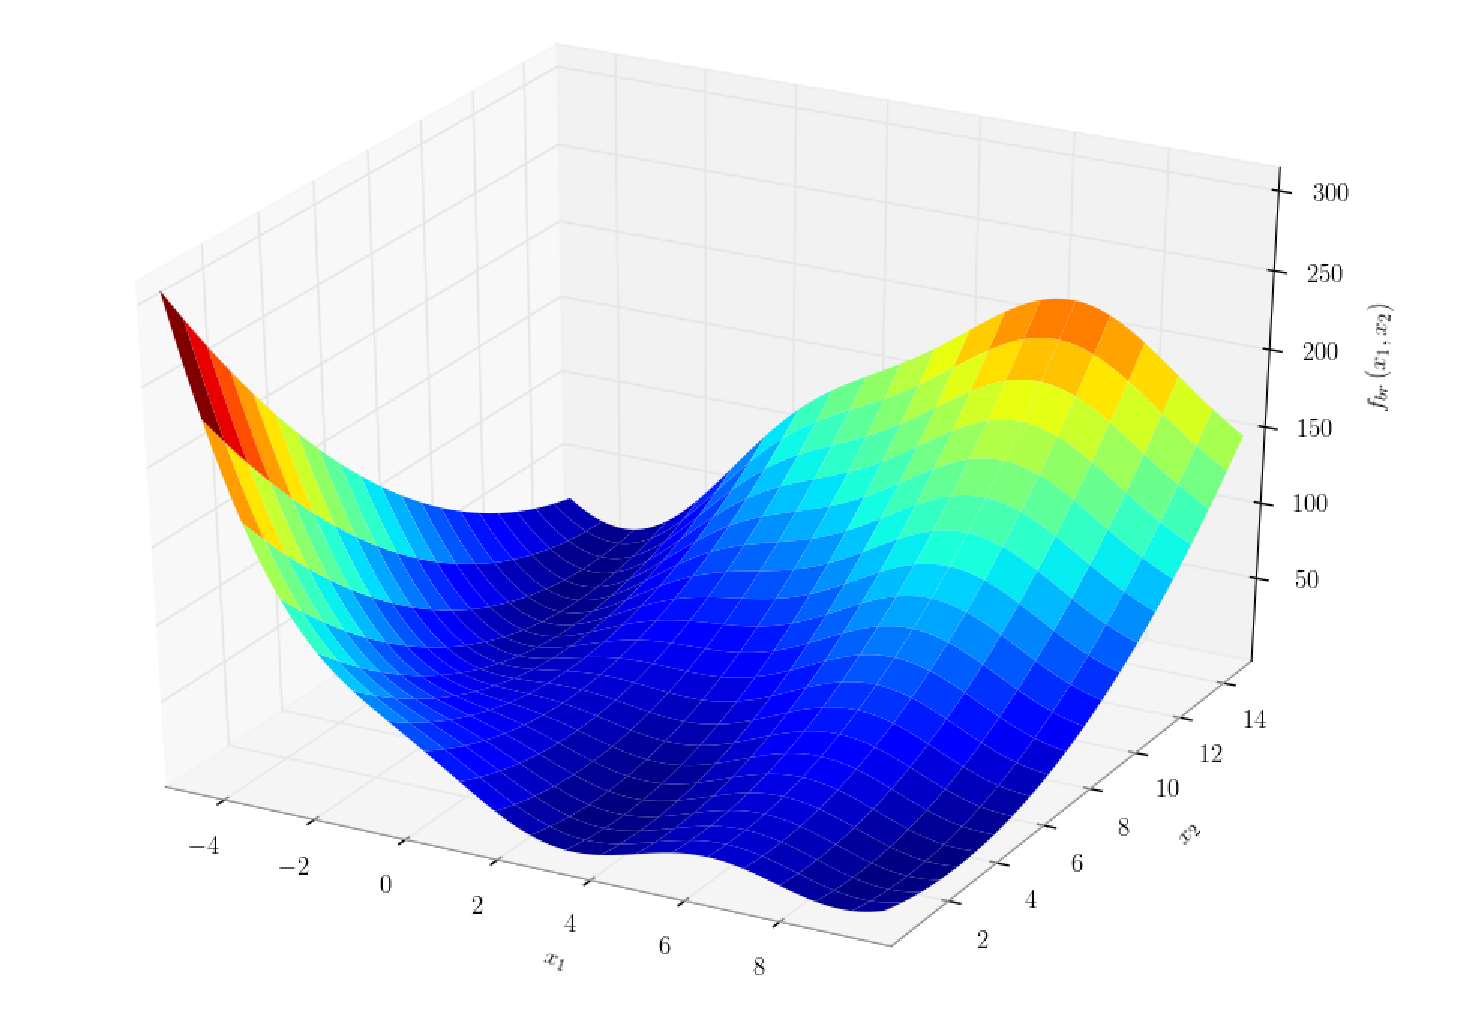
\includegraphics[width=\textwidth]{Chapter5/img/branin.pdf}
    \caption{Branin}
  \end{subfigure}
  \begin{subfigure}{0.24\textwidth}
    \centering\includegraphics[width=\textwidth]{Chapter5/img/himmelblau.pdf}
    \caption{Himmelblau}
  \end{subfigure}
  \begin{subfigure}{0.24\textwidth}
    \centering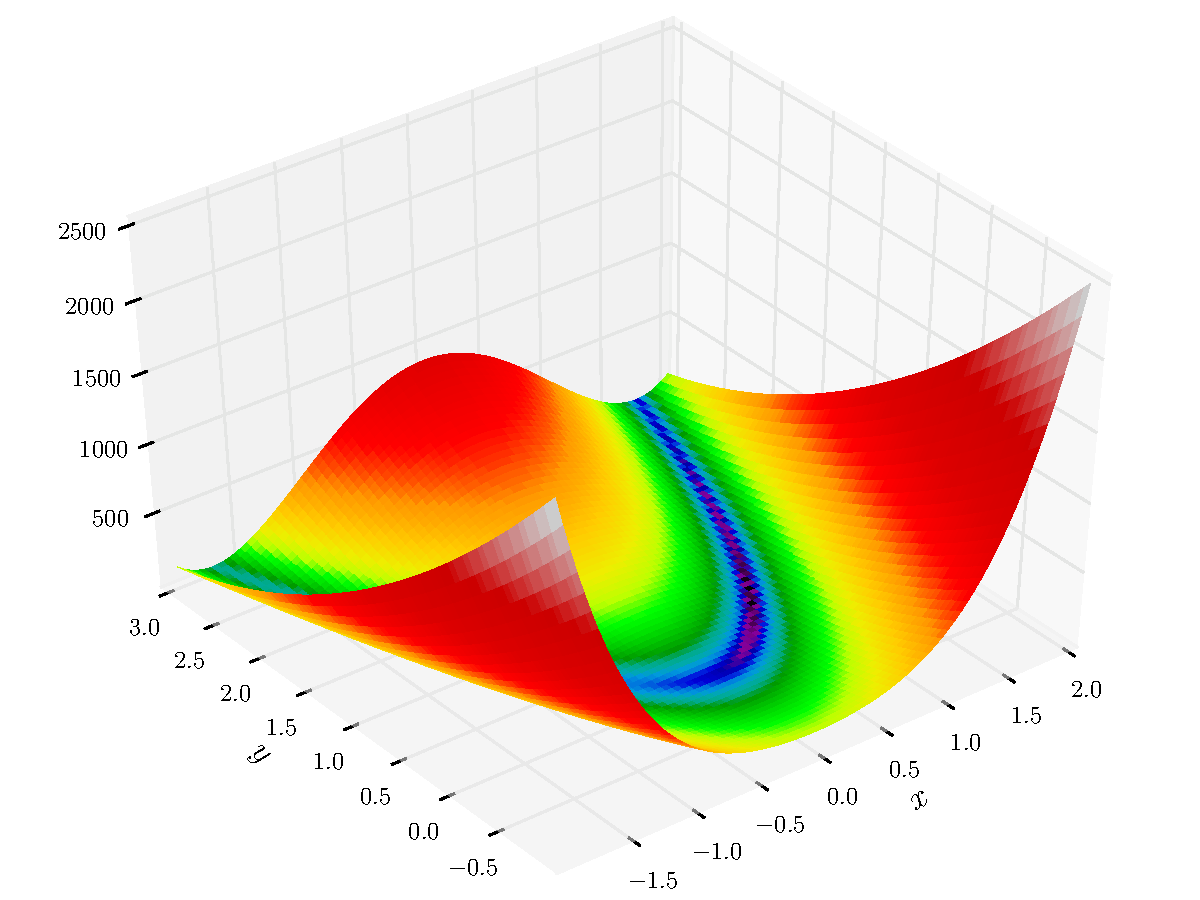
\includegraphics[width=\textwidth]{Chapter5/img/rosenbrock.pdf}
    \caption{Rosenbrock}
  \end{subfigure}
  \begin{subfigure}{0.24\textwidth}
    \centering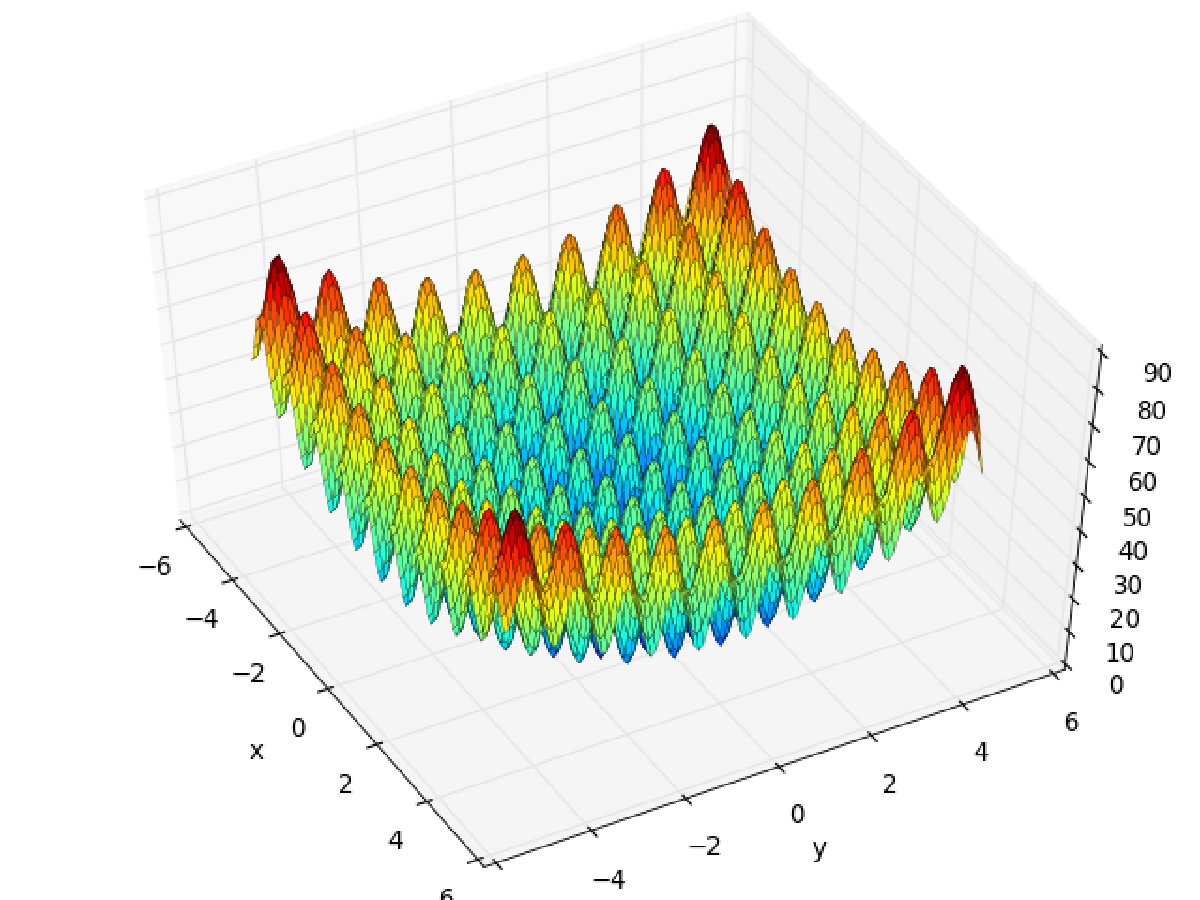
\includegraphics[width=\textwidth]{Chapter5/img/rastrigin.pdf}
    \caption{Rastrigin in 2D}
  \end{subfigure}
  \caption{Benchmark functions for testing black-box optimization algorithms.}
  \label{fig:benchmarks}
\end{figure}

\begin{figure}[ht]
  \centering
  \begin{subfigure}{0.49\textwidth}
    \centering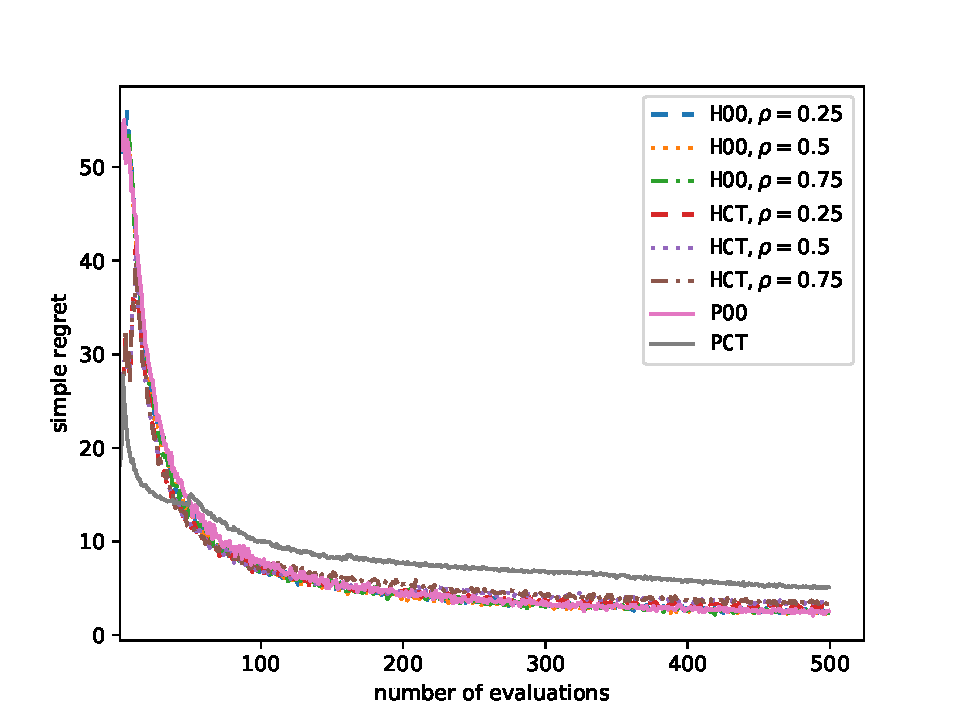
\includegraphics[width=\textwidth]{Chapter5/img/branin_plot.pdf}
    \caption{Branin}
  \end{subfigure}
  \begin{subfigure}{0.49\textwidth}
    \centering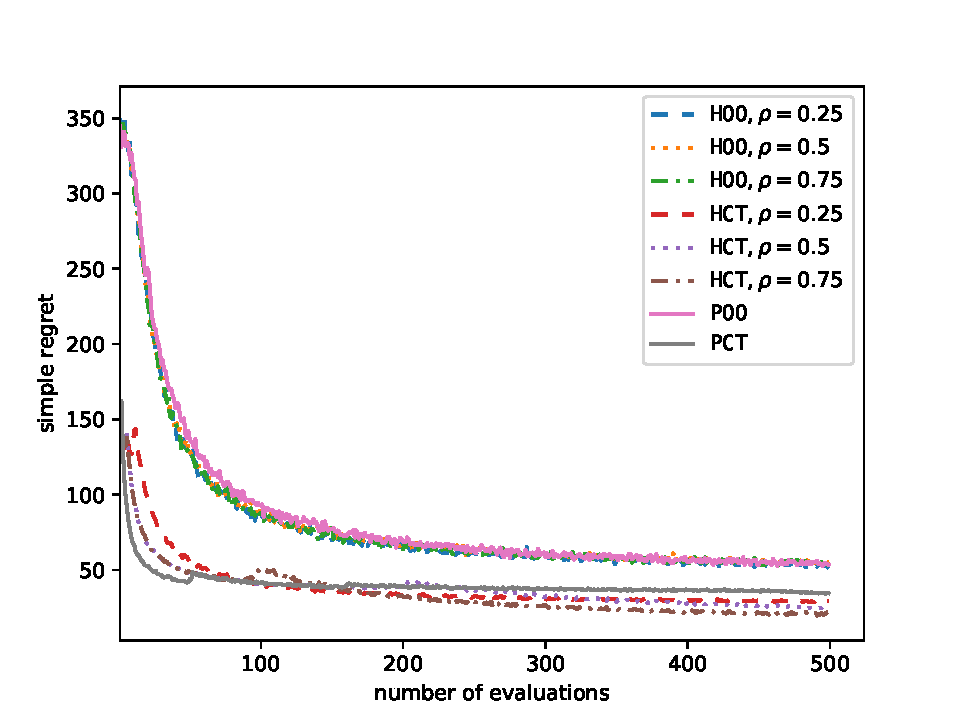
\includegraphics[width=\textwidth]{Chapter5/img/himmelblau_plot.pdf}
    \caption{Himmelblau}
  \end{subfigure}
  \begin{subfigure}{0.49\textwidth}
    \centering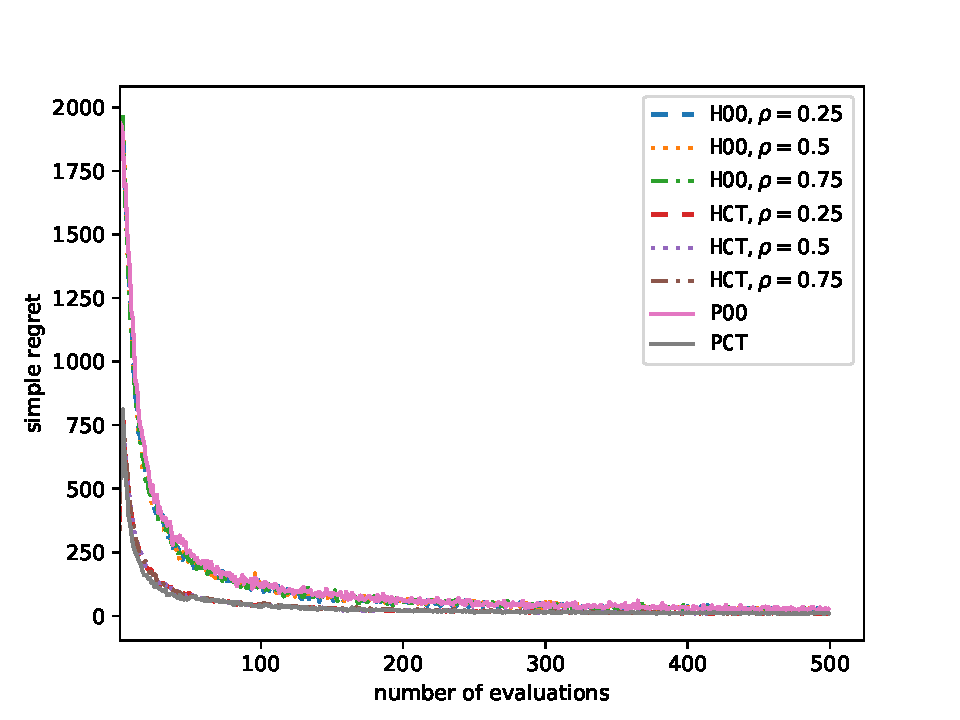
\includegraphics[width=\textwidth]{Chapter5/img/rosenbrock_plot.pdf}
    \caption{Rosenbrock}
  \end{subfigure}
  \begin{subfigure}{0.49\textwidth}
    \centering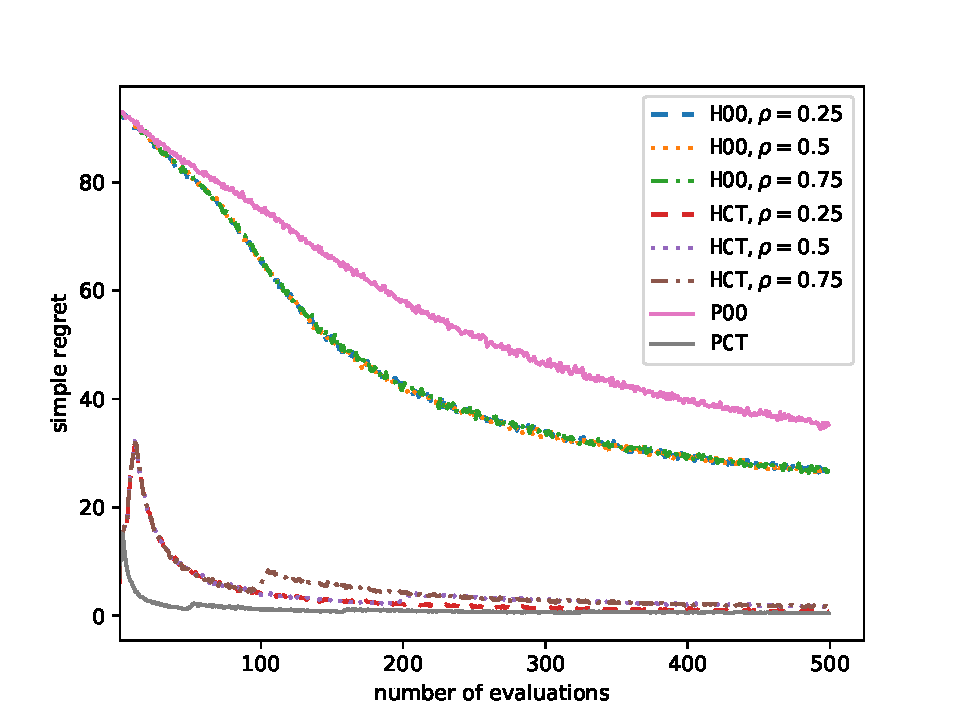
\includegraphics[width=\textwidth]{Chapter5/img/rastrigin_plot.pdf}
    \caption{Rastrigin in 5D}
  \end{subfigure}
  \caption{Simple regret of \POO and \PCT run for different $\rho$ values.}
  \label{fig:results}
\end{figure}

In Figure~\ref{fig:results}, we plot the simple regret of the algorithms as a function of the number of evaluations. All the results are averaged over 5000 runs and we plot the simple regret after 500 function evaluations. Each instance of \HOO or \HCT would recommend a point picked uniformly at random among those evaluated so that we have the same recommendation strategy as \POO and \PCT.

The first observation is that \PCT does match the performance of some single \HCT instances as expected. We also notice that \PCT has comparable performance w.r.t.\,\POO in these plots, which justifies the choice of using \HCT as a subroutine for the \POO meta-algorithm.
